\documentclass[conference,a4paper]{IEEEtran}
% ICAECA 2026: two-column A4, 4--6 pages including references, no page numbers.
\usepackage{cite}
\usepackage{amsmath,amssymb,amsfonts}
\usepackage{algorithm}
\usepackage{algorithmic}
\usepackage{graphicx}
\usepackage{textcomp}
\usepackage{xcolor}
\usepackage{booktabs}
\usepackage{url}
\usepackage{tikz}
\usetikzlibrary{arrows.meta,positioning,fit,backgrounds,calc}
\graphicspath{{figures/}}
% AUTO-GENERATED by gen_macros.py from the benchmark results -- do not edit by hand.
\newcommand{\EnrMeshTwo}{0.5}
\newcommand{\EnrMeshTwoPnf}{0.8}
\newcommand{\SyncMeshTwo}{4}
\newcommand{\SyncKiBMeshTwo}{10}
\newcommand{\EnrMeshThree}{1.4}
\newcommand{\EnrMeshThreePnf}{1.9}
\newcommand{\SyncMeshThree}{11}
\newcommand{\SyncKiBMeshThree}{40}
\newcommand{\EnrMeshFour}{2.4}
\newcommand{\EnrMeshFourPnf}{3.1}
\newcommand{\SyncMeshFour}{19}
\newcommand{\SyncKiBMeshFour}{92}
\newcommand{\EnrMeshSix}{5.3}
\newcommand{\EnrMeshSixPnf}{5.9}
\newcommand{\SyncMeshSix}{41}
\newcommand{\SyncKiBMeshSix}{301}
\newcommand{\EnrMeshEight}{8.6}
\newcommand{\EnrMeshEightPnf}{11.0}
\newcommand{\SyncMeshEight}{71}
\newcommand{\SyncKiBMeshEight}{702}
\newcommand{\EnrMeshTwelve}{24.1}
\newcommand{\EnrMeshTwelvePnf}{25.8}
\newcommand{\SyncMeshTwelve}{155}
\newcommand{\SyncKiBMeshTwelve}{2329}
\newcommand{\EnrMeshSixteen}{40.2}
\newcommand{\EnrMeshSixteenPnf}{42.0}
\newcommand{\SyncMeshSixteen}{271}
\newcommand{\SyncKiBMeshSixteen}{5472}
\newcommand{\EnrChainFour}{1.0}
\newcommand{\EnrChainFourPnf}{1.2}
\newcommand{\SyncChainFour}{9}
\newcommand{\SyncKiBChainFour}{42}
\newcommand{\EnrChainSix}{1.7}
\newcommand{\EnrChainSixPnf}{1.8}
\newcommand{\SyncChainSix}{13}
\newcommand{\SyncKiBChainSix}{91}
\newcommand{\EnrChainEight}{2.6}
\newcommand{\EnrChainEightPnf}{2.8}
\newcommand{\SyncChainEight}{17}
\newcommand{\SyncKiBChainEight}{161}
\newcommand{\EnrChainTwelve}{4.8}
\newcommand{\EnrChainTwelvePnf}{5.1}
\newcommand{\SyncChainTwelve}{25}
\newcommand{\SyncKiBChainTwelve}{363}
\newcommand{\EnrChainSixteen}{7.9}
\newcommand{\EnrChainSixteenPnf}{8.5}
\newcommand{\SyncChainSixteen}{33}
\newcommand{\SyncKiBChainSixteen}{649}
\newcommand{\RevMeshTwo}{0.6}
\newcommand{\RevMeshTwoPnf}{0.9}
\newcommand{\RevMsgsMeshTwo}{0}
\newcommand{\RevMeshThree}{0.8}
\newcommand{\RevMeshThreePnf}{1.1}
\newcommand{\RevMsgsMeshThree}{1}
\newcommand{\RevMeshFour}{1.0}
\newcommand{\RevMeshFourPnf}{1.5}
\newcommand{\RevMsgsMeshFour}{4}
\newcommand{\RevMeshSix}{1.4}
\newcommand{\RevMeshSixPnf}{1.6}
\newcommand{\RevMsgsMeshSix}{16}
\newcommand{\RevMeshEight}{2.0}
\newcommand{\RevMeshEightPnf}{2.6}
\newcommand{\RevMsgsMeshEight}{36}
\newcommand{\RevMeshTwelve}{4.1}
\newcommand{\RevMeshTwelvePnf}{4.5}
\newcommand{\RevMsgsMeshTwelve}{100}
\newcommand{\RevMeshSixteen}{6.6}
\newcommand{\RevMeshSixteenPnf}{7.9}
\newcommand{\RevMsgsMeshSixteen}{196}
\newcommand{\RevChainFour}{0.6}
\newcommand{\RevChainFourPnf}{1.1}
\newcommand{\RevMsgsChainFour}{2}
\newcommand{\RevChainSix}{1.0}
\newcommand{\RevChainSixPnf}{2.1}
\newcommand{\RevMsgsChainSix}{4}
\newcommand{\RevChainEight}{1.1}
\newcommand{\RevChainEightPnf}{2.6}
\newcommand{\RevMsgsChainEight}{6}
\newcommand{\RevChainTwelve}{1.7}
\newcommand{\RevChainTwelvePnf}{2.8}
\newcommand{\RevMsgsChainTwelve}{10}
\newcommand{\RevChainSixteen}{2.5}
\newcommand{\RevChainSixteenPnf}{3.8}
\newcommand{\RevMsgsChainSixteen}{14}
\newcommand{\AllDigestsAgree}{all}
\newcommand{\AEMsgsTwo}{4}
\newcommand{\AEMiBTwo}{0.0}
\newcommand{\AEMbpsTwo}{0.0}
\newcommand{\AEMsgsFour}{24}
\newcommand{\AEMiBFour}{0.1}
\newcommand{\AEMbpsFour}{0.5}
\newcommand{\AEMsgsEight}{112}
\newcommand{\AEMiBEight}{1.1}
\newcommand{\AEMbpsEight}{4.8}
\newcommand{\AEMsgsTwelve}{264}
\newcommand{\AEMiBTwelve}{4.0}
\newcommand{\AEMbpsTwelve}{16.8}
\newcommand{\AEMsgsSixteen}{480}
\newcommand{\AEMiBSixteen}{9.7}
\newcommand{\AEMbpsSixteen}{40.8}
\newcommand{\AETableRows}{2 & 4 & 10 & 0.04 & 0 \\
4 & 24 & 125 & 0.51 & 0 \\
8 & 112 & 1162 & 4.76 & 0 \\
12 & 264 & 4110 & 16.83 & 0 \\
16 & 480 & 9965 & 40.82 & 0 \\}
\newcommand{\BulkTableRows}{Loopback, unshaped & 3172 & 2717 & 1011 & 6.7 & 14.3 \\
300\,Mb/s, 2\,ms & 259 & 265 & 196 & 11.1 & 21.2 \\
100\,Mb/s, 0.5\,\% loss & 18.2 & 19.2 & 14.5 & 21.9 & 37.6 \\}
\newcommand{\LinkUnshapedGbps}{2.72}
\newcommand{\MuxUnshapedGbps}{1.01}
\newcommand{\UnshapedSpeedup}{2.7}
\newcommand{\CpuRatioUnshaped}{2.1}
\newcommand{\CpuRatioWifi}{1.9}
\newcommand{\LinkWifiMbps}{265.0}
\newcommand{\RawWifiMbps}{259.3}
\newcommand{\MuxWifiMbps}{195.6}
\newcommand{\MuxWifiLossPct}{26.2}
\newcommand{\LinkLossyMbps}{19.2}
\newcommand{\MuxLossyMbps}{14.5}
\newcommand{\RawLossyMbps}{18.2}
\newcommand{\InpUdpZeroPfifty}{12.1}
\newcommand{\InpUdpZeroPnn}{24.1}
\newcommand{\InpUdpZeroMax}{24.9}
\newcommand{\InpUdpZeroDel}{100.0}
\newcommand{\InpUdpZeroBulk}{168}
\newcommand{\InpUdpZeroEvents}{1850}
\newcommand{\InpTcpZeroPfifty}{13.2}
\newcommand{\InpTcpZeroPnn}{19.2}
\newcommand{\InpTcpZeroMax}{20.0}
\newcommand{\InpTcpZeroDel}{100.0}
\newcommand{\InpTcpZeroBulk}{184}
\newcommand{\InpTcpZeroEvents}{1855}
\newcommand{\InpMuxZeroPfifty}{72.7}
\newcommand{\InpMuxZeroPnn}{98.8}
\newcommand{\InpMuxZeroMax}{105.4}
\newcommand{\InpMuxZeroDel}{100.0}
\newcommand{\InpMuxZeroBulk}{125}
\newcommand{\InpMuxZeroEvents}{1788}
\newcommand{\InpUdpOnePfifty}{2.5}
\newcommand{\InpUdpOnePnn}{3.4}
\newcommand{\InpUdpOneMax}{4.0}
\newcommand{\InpUdpOneDel}{98.9}
\newcommand{\InpUdpOneBulk}{20}
\newcommand{\InpUdpOneEvents}{1843}
\newcommand{\InpTcpOnePfifty}{2.6}
\newcommand{\InpTcpOnePnn}{22.7}
\newcommand{\InpTcpOneMax}{41.1}
\newcommand{\InpTcpOneDel}{100.0}
\newcommand{\InpTcpOneBulk}{23}
\newcommand{\InpTcpOneEvents}{1840}
\newcommand{\InpMuxOnePfifty}{53.2}
\newcommand{\InpMuxOnePnn}{109.3}
\newcommand{\InpMuxOneMax}{139.1}
\newcommand{\InpMuxOneDel}{100.0}
\newcommand{\InpMuxOneBulk}{15}
\newcommand{\InpMuxOneEvents}{1842}
\newcommand{\InpUdpThreePfifty}{2.4}
\newcommand{\InpUdpThreePnn}{3.4}
\newcommand{\InpUdpThreeMax}{3.9}
\newcommand{\InpUdpThreeDel}{96.9}
\newcommand{\InpUdpThreeBulk}{10}
\newcommand{\InpUdpThreeEvents}{1835}
\newcommand{\InpTcpThreePfifty}{2.5}
\newcommand{\InpTcpThreePnn}{153.2}
\newcommand{\InpTcpThreeMax}{221.3}
\newcommand{\InpTcpThreeDel}{100.0}
\newcommand{\InpTcpThreeBulk}{10}
\newcommand{\InpTcpThreeEvents}{1835}
\newcommand{\InpMuxThreePfifty}{115.1}
\newcommand{\InpMuxThreePnn}{404.9}
\newcommand{\InpMuxThreeMax}{445.5}
\newcommand{\InpMuxThreeDel}{100.0}
\newcommand{\InpMuxThreeBulk}{7}
\newcommand{\InpMuxThreeEvents}{1835}
\newcommand{\PoolHashTwo}{12}
\newcommand{\PoolHashFour}{19}
\newcommand{\PoolHashEight}{35}
\newcommand{\PoolHashSixteen}{71}
\newcommand{\PoolHashThirtyTwo}{138}
\newcommand{\PoolHashSixtyFour}{263}
\newcommand{\SasUs}{1.1}
\newcommand{\FpUs}{3.9}
\newcommand{\GcmOpusUs}{10.0}
\newcommand{\GcmPcmUs}{11.9}
\newcommand{\OpusUs}{66}
\newcommand{\OpusBudgetPct}{0.76}
\newcommand{\OpusFrameBytes}{128}

\renewcommand{\algorithmicrequire}{\textbf{Input:}}
\newcommand{\T}{\mathcal{T}}
\newcommand{\V}{\mathcal{V}}
\newcommand{\PP}{\mathcal{P}}
% Start a new, centered row of author blocks (standard IEEEtran idiom).
\makeatletter
\newcommand{\linebreakand}{\end{@IEEEauthorhalign}\hfill\mbox{}\par\mbox{}\hfill\begin{@IEEEauthorhalign}}
\makeatother

\begin{document}

\title{A Secure Decentralized Cross-Device Communication and Synchronization Framework with Transitive Trust and Plane-Separated Transport}

\author{\IEEEauthorblockN{Ms. N. Nandhini}
\IEEEauthorblockA{\textit{Department of Computer Science}\\
\textit{and Engineering}\\
\textit{KPR Institute of Engineering}\\
\textit{and Technology}\\
Coimbatore, Tamil Nadu, India \\
nandhini.n@kpriet.ac.in}
\and
\IEEEauthorblockN{Dixit Tharun Raja P}
\IEEEauthorblockA{\textit{Department of Computer Science}\\
\textit{and Engineering}\\
\textit{KPR Institute of Engineering}\\
\textit{and Technology}\\
Coimbatore, Tamil Nadu, India \\
23cs044@kpriet.ac.in}
\and
\IEEEauthorblockN{Dharaneesh D}
\IEEEauthorblockA{\textit{Department of Computer Science}\\
\textit{and Engineering}\\
\textit{KPR Institute of Engineering}\\
\textit{and Technology}\\
Coimbatore, Tamil Nadu, India \\
23cs036@kpriet.ac.in}
\linebreakand
\IEEEauthorblockN{Deepanandham P}
\IEEEauthorblockA{\textit{Department of Computer Science}\\
\textit{and Engineering}\\
\textit{KPR Institute of Engineering}\\
\textit{and Technology}\\
Coimbatore, Tamil Nadu, India \\
23csl02@kpriet.ac.in}
\and
\IEEEauthorblockN{Gohul S}
\IEEEauthorblockA{\textit{Department of Computer Science}\\
\textit{and Engineering}\\
\textit{KPR Institute of Engineering}\\
\textit{and Technology}\\
Coimbatore, Tamil Nadu, India \\
23cs049@kpriet.ac.in}}

\maketitle
\pagestyle{empty}
\thispagestyle{empty}

\begin{abstract}
Personal computing now spans laptops, phones and televisions, yet the tools that connect these devices either depend on a vendor cloud account or require every pair of devices to be introduced separately. This paper presents Link, a zero-cloud framework that joins Windows and Android devices on a local network into a mutually authenticated device mesh. Link contributes a transitive trust-on-first-use enrollment protocol in which one human-verified pairing with any member admits a newcomer to the whole pool, a membership digest carried by heartbeats for anti-entropy repair, and flooded revocation. Traffic is separated into a persistent TLS control plane, an ephemeral certificate-pinned bulk plane with write back-pressure, and a UDP real-time plane for input events and AES-GCM protected Opus audio. The unmodified protocol implementation was evaluated under controlled network emulation. A sixteen-device pool converged after an enrollment in \EnrMeshSixteen~ms and purged a revoked device in \RevMeshSixteen~ms, while the number of human pairing ceremonies fell from quadratic to linear in the pool size. Computing the digest over the full membership view removed up to \AEMiBSixteen~MiB of redundant synchronization traffic per heartbeat. The bulk plane matched raw TCP goodput on a shaped 300~Mbps link with \CpuRatioWifi\ times lower CPU cost than Base64 transfer over the control channel, and the UDP plane bounded the 99th-percentile input latency at \InpUdpOnePnn~ms under one percent loss, against \InpMuxOnePnn~ms for a single multiplexed stream.
\end{abstract}

\begin{IEEEkeywords}
cross-device communication, peer-to-peer networks, trust on first use, device pairing, transport layer security, gossip protocols, local-first software, network security
\end{IEEEkeywords}

\section{Introduction}
A typical user now owns several computing devices and expects them to behave as one system: text copied on a phone should paste on a laptop, a file should move at local-network speed, and a phone should act as a touchpad, presenter or microphone for a nearby computer \cite{brudy2019crossdevice}. Commercial ecosystems deliver this experience by binding every device to a cloud account, which makes cross-device trust depend on an online identity provider and exposes metadata even when both devices share one room \cite{celosia2020discontinued, stute2019billion}. The local-first movement argues that such collaboration should work without a server and keep data under user control \cite{kleppmann2019localfirst}.

Open, serverless tools such as KDE Connect \cite{kdeconnect} avoid the cloud by pinning self-signed certificates on first use, but they introduce two practical costs. First, trust is strictly pairwise: a household with $N$ devices needs $N(N-1)/2$ separate pairing ceremonies, and removing a lost device requires visiting every other device. Second, a single control connection per device pair often carries notifications, clipboard data and input events together, so a lost segment or a large message delays everything behind it. Wireless LANs make this worse because loss and queueing delay vary widely under load \cite{liu2023wifi6, carrascosa2024mlo}.

This paper describes the design, implementation and evaluation of \emph{Link}, a framework that removes both costs while remaining fully local (Fig.~\ref{fig:arch}). Its contributions are as follows.
\begin{enumerate}
\item \textbf{Transitive trust-on-first-use (T-TOFU) enrollment.} One short-authentication-string (SAS) confirmation with any pool member enrolls a newcomer in the whole pool; membership views are repaired by digest-driven anti-entropy, and revocation is flooded to all members (Section~\ref{sec:trust}).
\item \textbf{Plane-separated transport.} Control, bulk and real-time traffic use a persistent TLS channel, one-shot pinned TLS channels with back-pressure, and UDP datagrams with per-session authenticated encryption, respectively (Section~\ref{sec:transport}).
\item \textbf{A cross-platform implementation} for Windows and Android that adds a user-mode file-system mount, input injection and audio relay on top of these planes.
\item \textbf{A reproducible evaluation} of the unmodified protocol code under network emulation, which also exposed two protocol defects and their correction (Sections~\ref{sec:eval} and~\ref{sec:security}).
\end{enumerate}

\begin{figure*}[t]
\centering
% Fig. 1 -- Link system architecture (vector TikZ, drawn at native \textwidth; no scaling).
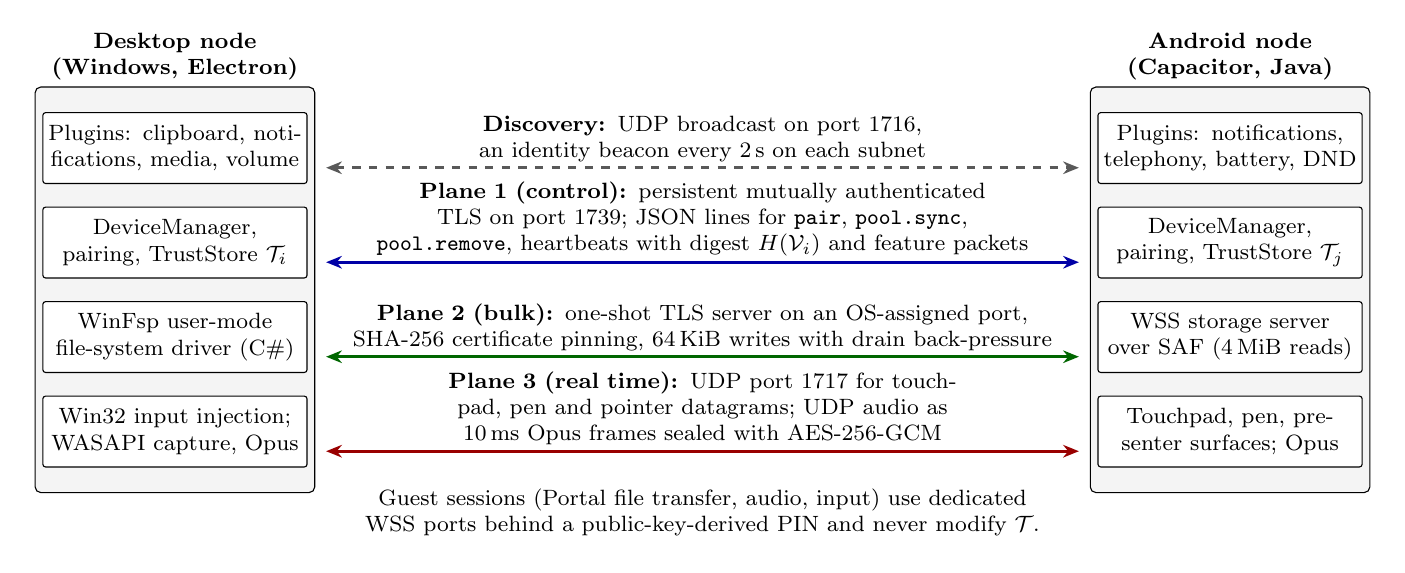
\begin{tikzpicture}[
  font=\footnotesize,
  >={Stealth[length=2mm,width=1.6mm]},
  mod/.style={draw, rounded corners=1pt, fill=white, text width=3.25cm, align=center,
              minimum height=0.9cm, inner sep=1.5pt},
  host/.style={draw, rounded corners=2pt, fill=gray!9, inner sep=0pt},
  hostlbl/.style={font=\footnotesize\bfseries, anchor=south, align=center, text width=3.6cm, inner sep=2pt},
  lane/.style={<->, line width=1.0pt},
  lbl/.style={align=center, text width=8.9cm, inner sep=0pt, anchor=south}
]
\def\xl{1.8}    % desktop column centre
\def\xr{15.2}   % android column centre
\def\ll{3.72}   % lane start
\def\lr{13.28}  % lane end
\foreach \y/\txt in {
  4.8/{Plugins: clipboard, notifications, media, volume},
  3.6/{DeviceManager, pairing, TrustStore $\mathcal{T}_i$},
  2.4/{WinFsp user-mode file-system driver (C\#)},
  1.2/{Win32 input injection; WASAPI capture, Opus}}
  \node[mod] at (\xl,\y) {\txt};
\foreach \y/\txt in {
  4.8/{Plugins: notifications, telephony, battery, DND},
  3.6/{DeviceManager, pairing, TrustStore $\mathcal{T}_j$},
  2.4/{WSS storage server over SAF (4\,MiB reads)},
  1.2/{Touchpad, pen, presenter surfaces; Opus}}
  \node[mod] at (\xr,\y) {\txt};
\begin{scope}[on background layer]
  \node[host, minimum width=3.55cm, minimum height=5.15cm] (D) at (\xl,3.0) {};
  \node[host, minimum width=3.55cm, minimum height=5.15cm] (A) at (\xr,3.0) {};
\end{scope}
\node[hostlbl] at (D.north) {Desktop node\\(Windows, Electron)};
\node[hostlbl] at (A.north) {Android node\\(Capacitor, Java)};
\draw[lane, dashed, gray!70!black] (\ll,4.55) -- (\lr,4.55);
\node[lbl] at ({(\ll+\lr)/2},4.62) {\textbf{Discovery:} UDP broadcast on port 1716, an identity beacon every 2\,s on each subnet};
\draw[lane, blue!65!black] (\ll,3.35) -- (\lr,3.35);
\node[lbl] at ({(\ll+\lr)/2},3.42) {\textbf{Plane 1 (control):} persistent mutually authenticated TLS on port 1739; JSON lines for \texttt{pair}, \texttt{pool.sync}, \texttt{pool.remove}, heartbeats with digest $H(\mathcal{V}_i)$ and feature packets};
\draw[lane, green!40!black] (\ll,2.15) -- (\lr,2.15);
\node[lbl] at ({(\ll+\lr)/2},2.22) {\textbf{Plane 2 (bulk):} one-shot TLS server on an OS-assigned port, SHA-256 certificate pinning, 64\,KiB writes with drain back-pressure};
\draw[lane, red!60!black] (\ll,0.95) -- (\lr,0.95);
\node[lbl] at ({(\ll+\lr)/2},1.02) {\textbf{Plane 3 (real time):} UDP port 1717 for touchpad, pen and pointer datagrams; UDP audio as 10\,ms Opus frames sealed with AES-256-GCM};
\node[font=\footnotesize, align=center, text width=9.2cm, anchor=north] at ({(\ll+\lr)/2},0.6) {Guest sessions (Portal file transfer, audio, input) use dedicated WSS ports behind a public-key-derived PIN and never modify $\mathcal{T}$.};
\end{tikzpicture}

\caption{Link architecture. Each traffic class has its own plane: persistent control TLS, one-shot pinned bulk TLS, and UDP for real-time input and encrypted audio.}
\label{fig:arch}
\end{figure*}

\section{Related Work}
\label{sec:related}
\textit{Vendor ecosystems and proximity protocols.} Apple Continuity and AirDrop rely on account-bound identities and proprietary radio protocols. Their continuity advertisements leak personal data \cite{celosia2020discontinued}, and the Apple Wireless Direct Link has been reverse engineered and shown to allow tracking, denial-of-service and man-in-the-middle attacks \cite{stute2019billion}. PrivateDrop repairs the contact-discovery leak of AirDrop with private set intersection \cite{heinrich2021privatedrop}. Bluetooth pairing, the other common proximity mechanism, remains exposed to key-downgrade attacks such as BLUFFS \cite{antonioli2023bluffs, casar2022ble}. Link avoids both account binding and proprietary radio layers by running over ordinary IP on the local network.

\textit{Serverless LAN tools and trust establishment.} KDE Connect \cite{kdeconnect} established the model that Link builds upon: UDP discovery, a JSON packet protocol over TLS, and pairwise trust on first use. Trust on first use is also the basis of SSH host authentication, where users rarely verify fingerprints \cite{neef2022ssh}, and certificate pinning is the standard defense when a public PKI is absent \cite{pradeep2022pinning}. Syncthing lets a designated introducer device share its device list \cite{syncthingintroducer}. Link differs by making every member an introducer, by detecting divergence through a membership digest, and by propagating revocation. The design follows zero-trust principles in that the network location grants no privilege \cite{nist80207, nahar2024zerotrust}, and it complements identity-centric IoT approaches that anchor TLS in self-sovereign credentials \cite{perugini2024ssi}.

\textit{Membership dissemination and transport.} Epidemic protocols spread updates by anti-entropy and rumor mongering \cite{demers1987epidemic}, and recent work adapts gossip membership to constrained edge devices \cite{daubaris2026muswim}. QUIC removes transport head-of-line blocking between streams \cite{rfc9000} and is being evaluated as the multiplexing layer of WebRTC \cite{engelbart2026quic}; Link instead separates traffic classes onto existing TLS and UDP sockets, which are available on every target platform without an extra protocol stack. Table~\ref{tab:compare} summarizes the positioning.

\begin{table}[t]
\caption{Positioning of Link Against Representative Systems}
\label{tab:compare}
\centering
\footnotesize
\setlength{\tabcolsep}{2pt}
\begin{tabular}{@{}lcccc@{}}
\toprule
Property & KDE Connect & Apple & Quick Share & \textbf{Link} \\
\midrule
Cloud account needed & No & Yes & Yes$^{a}$ & \textbf{No} \\
Ceremonies, $N$ devices & $\binom{N}{2}$ & account & account & $\mathbf{N-1}$ \\
Pool-wide revocation & No & account & account & \textbf{Yes} \\
Separate bulk channel & Yes & Yes & Yes & \textbf{Yes} \\
UDP real-time input & No & n/d$^{b}$ & n/a & \textbf{Yes} \\
Unenrolled guests & No & Yes & Yes & \textbf{Yes} \\
\bottomrule
\multicolumn{5}{@{}l}{\scriptsize $^{a}$``Your devices'' mode. $^{b}$Not publicly documented.}\\
\multicolumn{5}{@{}l}{\scriptsize n/a: feature not offered.}
\end{tabular}
\end{table}

\section{System and Threat Model}
\label{sec:model}
A \emph{pool} $\PP$ is the set of devices owned by one user. Each device $d_i$ has a random 128-bit identifier and a long-lived self-signed X.509 certificate $C_i$ with an RSA-2048 key $K_i$; its fingerprint is
\begin{equation}
f_i=\mathrm{SHA\text{-}256}(\mathrm{DER}(C_i)).
\end{equation}
Device $d_i$ keeps a trust store $\T_i$ of $(d_j,C_j)$ entries, encrypted at rest with the operating-system key store on the desktop. Its \emph{membership view} includes itself:
\begin{equation}
\V_i=\T_i\cup\{(d_i,C_i)\}.
\end{equation}
The pool is consistent when $\V_i=\PP$ for every member.

The adversary controls the local network: it can observe, drop, delay, replay and inject packets, run its own devices and answer discovery broadcasts, but it cannot compromise the operating system of a member or read its private key. The user compares a short authentication string exactly once when a device joins. The goals are (G1) authenticity and confidentiality of control and bulk traffic, (G2) admission of new members only through a human-confirmed pairing with an existing member, (G3) eventual consistency of membership views, and (G4) timely, pool-wide revocation.

\section{Transitive Trust Enrollment}
\label{sec:trust}
\subsection{Discovery, Connection and Pairing}
Every device broadcasts an identity beacon every 2~s to the broadcast address of each attached subnet (UDP port 1716). On discovery, peers open a mutually authenticated TLS~1.2/1.3 connection (port 1739), which the desktop restricts to AEAD cipher suites \cite{rfc8446}. Chain validation is intentionally disabled because certificates are self-signed; instead, after the identity packet reveals the claimed $d_j$, the receiver compares the presented fingerprint with the pinned $f_j$ and closes the connection on mismatch. When two peers dial each other simultaneously, both keep the same socket without negotiation by the rule
\begin{equation}
\text{keep outbound}\iff d_{\mathrm{local}}<d_{\mathrm{remote}},
\end{equation}
evaluated lexicographically on the identifiers.

Pairing a stranger is a four-state machine (not paired, requested, requested by peer, paired) with a 30~s timeout and a 30~min bound on clock skew. Both devices display
\begin{equation}
\mathrm{SAS}=\mathrm{Trunc}_{32}\big(\mathrm{SHA\text{-}256}(K_{\max}\,\Vert\,K_{\min}\,\Vert\,\tau)\big),
\end{equation}
as eight hexadecimal characters, where $K_{\max}$ and $K_{\min}$ are the two DER-encoded public keys in byte order and $\tau$ is the request timestamp. A man-in-the-middle who substitutes either key changes the string with probability $1-2^{-32}$.

\subsection{Membership Views and Anti-Entropy}
Algorithm~\ref{alg:pool} gives the per-device logic. After a confirmed pairing, both devices insert each other and broadcast their views in \texttt{pool.sync} messages. A receiver adds every unknown entry, upgrades any open connection whose presented certificate matches the newly pinned one, and rebroadcasts only when its own view changed. The rule in line~\ref{line:trusted} is essential: a view is accepted only from a peer that is already trusted over an authenticated channel, so that transitive trust never originates from a stranger.

Divergence caused by partitions or lost messages is repaired by anti-entropy. Every heartbeat (2~s) carries the digest
\begin{equation}
H(\V)=\mathrm{Trunc}_{64}\Big(\mathrm{SHA\text{-}256}\big(\textstyle\big\Vert_{(d,C)\in\mathrm{sort}(\V)} d\,{:}\,f(C)\,{\mid}\big)\Big),
\end{equation}
and a trusted receiver whose own digest differs replies with its view. Because two consistent members hold the same set $\V_i=\V_j=\PP$, their digests are equal and a converged pool exchanges no synchronization traffic.

\begin{algorithm}[t]
\caption{Pool maintenance at device $d_i$}
\label{alg:pool}
\begin{algorithmic}[1]
\small
\REQUIRE trust store $\T_i$, connections with trust flags
\STATE \textbf{on} pairing confirmed with $(d_p,C_p)$:
\STATE \quad $\T_i\gets\T_i\cup\{(d_p,C_p)\}$; \textsc{Broadcast}$(\V_i)$
\STATE \textbf{on} message $m$ from peer $d_s$:
\IF{$m$ is \texttt{pool.sync} or \texttt{pool.remove} \textbf{and} $d_s$ not trusted}
  \STATE drop $m$ \label{line:trusted}
\ELSIF{$m=\texttt{pool.sync}(L)$}
  \STATE $\mathit{chg}\gets\FALSE$
  \FORALL{$(d,C)\in L$ with $d\neq d_i$ and $d\notin\T_i$}
    \STATE $\T_i\gets\T_i\cup\{(d,C)\}$; $\mathit{chg}\gets\TRUE$
    \STATE \textbf{if} a connection to $d$ presents $f(C)$ \textbf{then} mark it trusted
  \ENDFOR
  \STATE \textbf{if} $\mathit{chg}$ \textbf{then} \textsc{Broadcast}$(\V_i)$
\ELSIF{$m=\texttt{heartbeat}(h)$ and $h\neq H(\V_i)$}
  \STATE send $\texttt{pool.sync}(\V_i)$ to $d_s$
\ELSIF{$m=\texttt{pool.remove}(d_x)$ and $d_x\in\T_i$}
  \STATE $\T_i\gets\T_i\setminus\{d_x\}$; send \texttt{pair}(\textit{false}) to $d_x$; close
  \STATE forward $m$ to every trusted peer $\notin\{d_s,d_x\}$
\ENDIF
\STATE \textbf{procedure} \textsc{Broadcast}$(\V)$: send $\texttt{pool.sync}(\V)$ to all trusted peers
\end{algorithmic}
\end{algorithm}

\begin{figure}[t]
\centering
% Fig. 2 -- Transitive enrollment and cascaded revocation (vector TikZ, native \columnwidth).
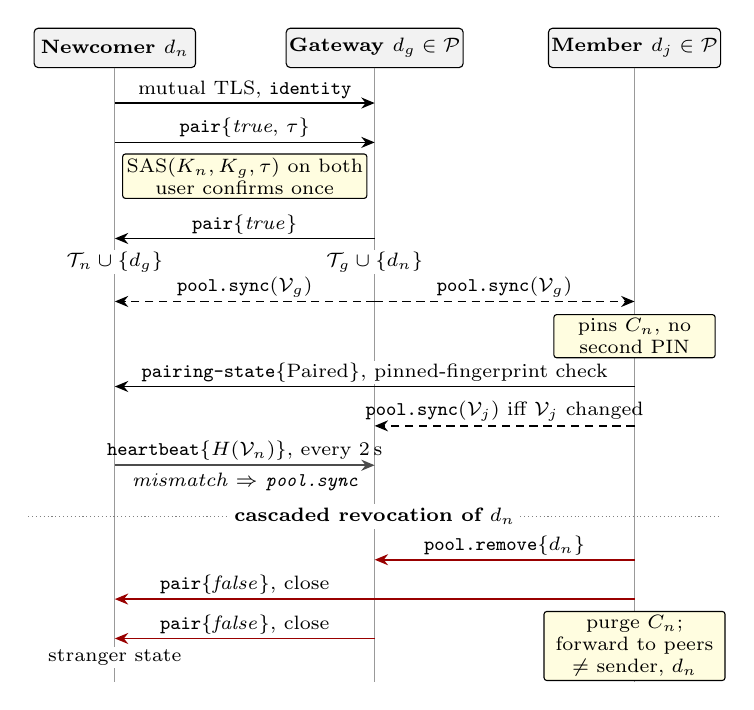
\begin{tikzpicture}[
  font=\scriptsize,
  >={Stealth[length=1.7mm,width=1.4mm]},
  actor/.style={draw, rounded corners=1.5pt, fill=gray!10, minimum width=2.05cm, minimum height=0.5cm,
                align=center, font=\scriptsize\bfseries, inner sep=1pt},
  msg/.style={->, line width=0.6pt},
  gossip/.style={->, line width=0.6pt, densely dashed},
  lbl/.style={inner sep=0.6pt, align=center, anchor=south},
  note/.style={draw, fill=yellow!12, rounded corners=1pt, align=center, inner sep=1.4pt}
]
\def\xn{1.05} \def\xg{4.35} \def\xj{7.65} \def\ybot{-8.05}
\node[actor] at (\xn,0) {Newcomer $d_n$};
\node[actor] at (\xg,0) {Gateway $d_g\in\mathcal{P}$};
\node[actor] at (\xj,0) {Member $d_j\in\mathcal{P}$};
\foreach \x in {\xn,\xg,\xj} \draw[gray!80, line width=0.4pt] (\x,-0.25) -- (\x,\ybot);
% ---------------- enrollment ----------------
\draw[msg] (\xn,-0.7) -- (\xg,-0.7);
\node[lbl] at ({(\xn+\xg)/2},-0.67) {mutual TLS, \texttt{identity}};
\draw[msg] (\xn,-1.2) -- (\xg,-1.2);
\node[lbl] at ({(\xn+\xg)/2},-1.17) {\texttt{pair}\{\textit{true}, $\tau$\}};
\node[note, align=center, anchor=north] at ({(\xn+\xg)/2},-1.34) {$\mathrm{SAS}(K_n,K_g,\tau)$ on both\\user confirms once};
\draw[msg] (\xg,-2.42) -- (\xn,-2.42);
\node[lbl] at ({(\xn+\xg)/2},-2.39) {\texttt{pair}\{\textit{true}\}};
\node[fill=white, inner sep=0.6pt] at (\xn,-2.72) {$\mathcal{T}_n\cup\{d_g\}$};
\node[fill=white, inner sep=0.6pt] at (\xg,-2.72) {$\mathcal{T}_g\cup\{d_n\}$};
\draw[gossip] (\xg,-3.22) -- (\xn,-3.22);
\node[lbl] at ({(\xn+\xg)/2},-3.19) {\texttt{pool.sync}$(\mathcal{V}_g)$};
\draw[gossip] (\xg,-3.22) -- (\xj,-3.22);
\node[lbl] at ({(\xg+\xj)/2},-3.19) {\texttt{pool.sync}$(\mathcal{V}_g)$};
\node[note, text width=1.95cm, anchor=north] at (\xj,-3.38) {pins $C_n$, no second PIN};
\draw[msg] (\xj,-4.3) -- (\xn,-4.3);
\node[lbl, fill=white] at ({(\xn+\xj)/2},-4.27) {\texttt{pairing-state}\{Paired\}, pinned-fingerprint check};
\draw[gossip] (\xj,-4.8) -- (\xg,-4.8);
\node[lbl] at ({(\xg+\xj)/2},-4.77) {\texttt{pool.sync}$(\mathcal{V}_j)$ iff $\mathcal{V}_j$ changed};
\draw[msg, gray!60!black] (\xn,-5.3) -- (\xg,-5.3);
\node[lbl] at ({(\xn+\xg)/2},-5.27) {\texttt{heartbeat}\{$H(\mathcal{V}_n)$\}, every 2\,s};
\node[anchor=north, align=center, font=\scriptsize\itshape, inner sep=1pt] at ({(\xn+\xg)/2},-5.36) {mismatch $\Rightarrow$ \texttt{pool.sync}};
% ---------------- revocation ----------------
\draw[gray, densely dotted] (-0.05,-5.95) -- (8.75,-5.95);
\node[fill=white, inner sep=1.5pt, font=\scriptsize\bfseries] at (\xg,-5.95) {cascaded revocation of $d_n$};
\draw[msg, red!60!black] (\xj,-6.5) -- (\xg,-6.5);
\node[lbl] at ({(\xg+\xj)/2},-6.47) {\texttt{pool.remove}\{$d_n$\}};
\draw[msg, red!60!black] (\xj,-7.0) -- (\xn,-7.0);
\node[lbl, fill=white] at ({(\xn+\xg)/2},-6.97) {\texttt{pair}\{\textit{false}\}, close};
\draw[msg, red!60!black] (\xg,-7.5) -- (\xn,-7.5);
\node[lbl] at ({(\xn+\xg)/2},-7.47) {\texttt{pair}\{\textit{false}\}, close};
\node[note, text width=2.2cm, anchor=north] at (\xj,-7.15) {purge $C_n$; forward to peers $\neq$ sender, $d_n$};
\node[anchor=north, fill=white, inner sep=1pt] at (\xn,-7.6) {stranger state};
\end{tikzpicture}

\caption{Transitive enrollment of $d_n$ through gateway $d_g$ (top) and cascaded revocation (bottom). Dashed arrows are gossip; only the first pairing needs a human.}
\label{fig:seq}
\end{figure}

\subsection{Cascaded Revocation}
Any member may revoke $d_x$ by sending \texttt{pool.remove} to its trusted peers and unpairing locally. Each receiver that still holds $d_x$ purges it, tells $d_x$ to unpair, closes the connection, and forwards the message to its other trusted peers (Fig.~\ref{fig:seq}). Forwarding happens only on the first removal, so duplicates die out; in a full mesh the flood costs $(N-2)^2$ messages of about 100~bytes.

\subsection{Properties}
\textit{Human effort.} Pairwise TOFU needs $E_{\mathrm{pw}}(N)=N(N-1)/2$ ceremonies to connect $N$ devices, while T-TOFU needs
\begin{equation}
E_{\mathrm{T}}(N)=N-1,
\end{equation}
one per newcomer; for $N=8$ this is 7 instead of 28.

\textit{Termination and convergence.} During enrollment the views only grow and are bounded by $\PP$, and a device rebroadcasts only after a change, so each device sends at most $|\PP|$ broadcasts and gossip terminates. If the graph of trusted connections is connected, induction on the hop distance from the gateway shows that every member eventually holds $\PP$; the heartbeat digest additionally repairs any loss.

\section{Plane-Separated Transport and OS Integration}
\label{sec:transport}
Fig.~\ref{fig:arch} shows how Link assigns each traffic class to its own plane so that a slow or lossy class cannot delay another.


\textit{Plane 1 (control).} The persistent TLS connection carries newline-delimited JSON packets for pairing, membership, heartbeats and low-rate feature messages (notifications, battery, telephony, media and volume state). A peer silent for 5~s is declared dead.

\textit{Plane 2 (bulk).} Files, clipboard images and speed tests never travel inside control packets. Following the payload model of KDE Connect \cite{kdeconnect}, the sender opens a one-shot TLS server on an OS-assigned port and announces the port in a control packet; the receiver connects and verifies the pinned fingerprint before reading (Algorithm~\ref{alg:bulk}). Link streams raw bytes in 64~KiB writes and suspends on socket back-pressure, and the Android receiver reads through a 128~KiB buffer. In field tests on the team's Wi-Fi network, replacing a single large write with this loop raised application throughput from about 80~Mbps to the roughly 220~Mbps ceiling measured for raw TCP on the same link.

\begin{algorithm}[t]
\caption{One-shot bulk transfer on Plane 2}
\label{alg:bulk}
\begin{algorithmic}[1]
\small
\REQUIRE payload $B$, pinned fingerprint $f_s$ of the sender
\STATE \textit{Sender:} $p\gets$ listen on TLS port 0; send \texttt{payload}$(|B|,p)$ on Plane 1
\STATE \textit{Receiver:} connect to $(\mathit{ip}_s,p)$; \textbf{if} $f(C_{\mathrm{presented}})\neq f_s$ \textbf{then} abort
\STATE \textit{Sender:} $o\gets0$
\WHILE{$o<|B|$}
  \STATE $\mathit{ok}\gets$ \textsc{Write}$(B[o\,..\,o+64\,\mathrm{KiB}])$; $o\gets o+64\,\mathrm{KiB}$
  \STATE \textbf{if not} $\mathit{ok}$ \textbf{then} wait for the \texttt{drain} event
\ENDWHILE
\STATE \textit{Sender:} end the stream and close the listener (one connection only)
\end{algorithmic}
\end{algorithm}

\textit{Plane 3 (real time).} Touchpad, pen and presenter events travel as small UDP datagrams (port 1717) that are accepted only from the address of a trusted or admitted peer. A lost datagram is simply superseded by the next one, which suits relative pointer motion. Relative deltas are injected with a sub-pixel carry $c$ so that slow finger motion is not rounded away:
\begin{equation}
\delta_{\mathrm{int}}=\mathrm{round}(\delta+c),\qquad c\gets\delta+c-\delta_{\mathrm{int}}.
\end{equation}
Audio relay encodes 10~ms Opus frames \cite{rfc6716} and seals each datagram with AES-256-GCM under a per-listener key delivered over TLS. The frame layout is sequence (4~B), capture timestamp (6~B), nonce (12~B), ciphertext of a codec tag and payload, and tag (16~B), i.e., 39~bytes of overhead; a reorder buffer and the timestamps drive the playback-rate correction. The same pipeline, reversed, exposes a phone microphone to the desktop.

\textit{OS integration and guests.} A WinFsp user-mode driver \cite{winfsp} mounts phone storage as a Windows drive. The driver talks to a token-protected loopback API, which reads 4~MiB chunks from the Android storage server over four pooled secure WebSocket connections, keeps a 512~MiB least-recently-used read cache and writes synchronously so that Explorer reports real progress. Unenrolled guests (Portal file transfer, audio, input) connect to dedicated ports, show a PIN derived from both public keys, and never modify any trust store.

\textit{Implementation.} The desktop client uses Electron and TypeScript (about 30~k lines including the user interface) with a C\# driver; the Android client uses Capacitor and Java (about 18~k lines). Clipboard, notification, telephony, media, volume, lock, input, file and audio features were verified end to end between a Windows desktop and Android phones on a real Wi-Fi LAN.

\section{Evaluation}
\label{sec:eval}
\subsection{Methodology}
All experiments execute the unmodified desktop protocol modules (device manager, trust store, pairing, transport and the bulk-transfer routine), bundled for Node.js 22.17 and run on an AMD Ryzen 7 5800H with 16~GB of memory under Linux 6.8. Transport experiments run each endpoint in its own process inside a private network namespace whose loopback interface is shaped by Linux \texttt{netem} with a 1500-byte MTU, so that loss, delay and rate limits act on real kernel TCP and UDP. Trust experiments run $N$ devices with real TLS connections in one process with trust stores on tmpfs, which isolates protocol cost from storage and radio latency. They use 20 trials per full-mesh configuration and 10 per chain. The trusted-sender rule and the view digest of Section~\ref{sec:trust} are applied as harness-level patches (Section~\ref{sec:security}); the harness and raw data accompany the source code.

\subsection{Enrollment, Revocation and Anti-Entropy}
Fig.~\ref{fig:conv} reports the median time from the gateway's confirmation until every member trusts the newcomer and every connection is upgraded, and the time from a revocation until every remaining member has purged the device. A full mesh of 8 devices converged in \EnrMeshEight~ms and one of 16 devices in \EnrMeshSixteen~ms, with 95th percentiles of \EnrMeshEightPnf~ms and \EnrMeshSixteenPnf~ms. Growth is superlinear because each learner rebroadcasts its full view, giving \SyncMeshSixteen\ messages (\SyncKiBMeshSixteen~KiB) for $N=16$; a chain, where the view must travel $N-2$ hops, needed only \EnrChainSixteen~ms because it has fewer links. Revocation completed in \RevMeshSixteen~ms (full mesh, \RevMsgsMeshSixteen\ messages) and \RevChainSixteen~ms (chain) for $N=16$. The newly computed digests were identical on all members in \AllDigestsAgree\ trials. These times are far below the 2~s heartbeat, so anti-entropy serves only as a repair path.

\begin{figure}[t]
\centering
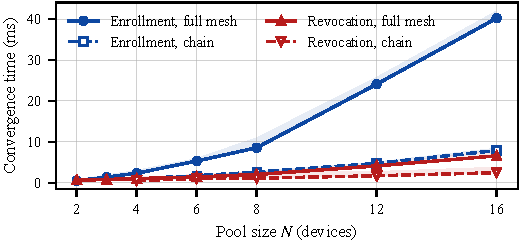
\includegraphics[width=\columnwidth]{fig_convergence.pdf}
\caption{Median convergence time versus pool size; shading extends to the 95th percentile.}
\label{fig:conv}
\end{figure}

Table~\ref{tab:ae} compares the idle heartbeat traffic of a converged full mesh for the original digest, which the prototype computed over $\T_i$, with the view digest $H(\V_i)$. Because $\T_i$ never contains $d_i$, two members never agree, so every heartbeat exchange triggered two full view transfers, i.e., $2N(N-1)$ messages per cycle. For 16 devices that is \AEMiBSixteen~MiB every 2~s, a constant \AEMbpsSixteen~Mbps of Wi-Fi airtime, whereas the view digest sends nothing.

\begin{table}[t]
\caption{Idle Synchronization Traffic per 2\,s Heartbeat Cycle}
\label{tab:ae}
\centering
\footnotesize
\begin{tabular}{@{}rrrrr@{}}
\toprule
& \multicolumn{3}{c}{Digest over $\T_i$ (original)} & $H(\V_i)$ \\
\cmidrule(lr){2-4}\cmidrule(l){5-5}
$N$ & messages & KiB & Mbps & messages \\
\midrule
\AETableRows
\bottomrule
\end{tabular}
\end{table}

\subsection{Bulk Plane Goodput and CPU Cost}
Table~\ref{tab:bulk} compares Plane~2 with raw TCP without encryption, an upper bound, and with the common alternative of sending Base64 chunks inside control-channel JSON packets (B64). On unshaped loopback, where CPU is the limit, Plane~2 reached \LinkUnshapedGbps~Gbps, \UnshapedSpeedup\ times the Base64 design, at \CpuRatioUnshaped\ times lower CPU cost per GiB. On a 300~Mbps link Plane~2 delivered \LinkWifiMbps~Mbps, equal to raw TCP (\RawWifiMbps~Mbps), whereas Base64 lost \MuxWifiLossPct\,\% of the goodput to the 4/3 encoding expansion. With 0.5\,\% random loss on a 100~Mbps link, TCP loss recovery limited every method to about \LinkLossyMbps~Mbps, and the ordering was unchanged.

\begin{table}[t]
\caption{Bulk Goodput and CPU Cost of Raw TCP, Link Plane~2 and Base64 in Control Packets (B64), Mean of 3 Runs}
\label{tab:bulk}
\centering
\footnotesize
\setlength{\tabcolsep}{4pt}
\begin{tabular}{@{}lrrrrr@{}}
\toprule
& \multicolumn{3}{c}{Goodput (Mbps)} & \multicolumn{2}{c}{CPU (s/GiB)} \\
\cmidrule(lr){2-4}\cmidrule(l){5-6}
Link condition & Raw & Link & B64 & Link & B64 \\
\midrule
\BulkTableRows
\bottomrule
\end{tabular}
\end{table}

\subsection{Input Latency Under Concurrent Load}
A sender emitted pointer events at 120~Hz for 15~s while a bulk transfer saturated a 200~Mbps link with 2$\pm$1~ms delay and a 400-packet queue. Three designs were compared: Link's UDP plane, a dedicated TCP control connection with Nagle's algorithm disabled, and a single TLS stream that also carries the bulk data. Fig.~\ref{fig:lat} shows the distributions. Random loss also throttles the competing TCP bulk flow and drains the queue, so the differences under loss stem from retransmission and in-stream ordering. At 1\,\% loss the 99th-percentile latency was \InpUdpOnePnn~ms for UDP, \InpTcpOnePnn~ms for dedicated TCP and \InpMuxOnePnn~ms for the multiplexed stream; at 3\,\% loss the values were \InpUdpThreePnn, \InpTcpThreePnn\ and \InpMuxThreePnn~ms. UDP delivered \InpUdpOneDel\,\% and \InpUdpThreeDel\,\% of the events, respectively; a lost relative-motion event is superseded 8~ms later, whereas a retransmission stalls all later events. Without loss the bulk flow keeps the queue full, so UDP and dedicated TCP both reach about 20~ms at the 99th percentile (\InpUdpZeroPnn\ and \InpTcpZeroPnn~ms) and the multiplexed stream \InpMuxZeroPnn~ms; plane separation removes head-of-line blocking inside a flow but not queueing at the access point.

\begin{figure*}[t]
\centering
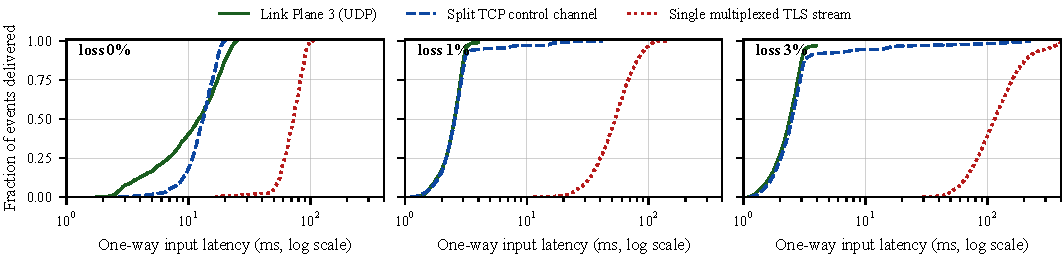
\includegraphics[width=\textwidth]{fig_latency_cdf.pdf}
\caption{Distribution of one-way input latency with a concurrent bulk transfer on a 200~Mbps link. Curves are normalized to the events sent, so a plateau below 1 indicates lost events.}
\label{fig:lat}
\end{figure*}

\subsection{Cost of the Security Primitives}
Computing $H(\V)$ took \PoolHashSixteen~$\mu$s for 16 members and \PoolHashSixtyFour~$\mu$s for 64, the SAS \SasUs~$\mu$s, and sealing plus opening one 10~ms audio frame with AES-256-GCM \GcmOpusUs~$\mu$s. Opus encoding and decoding of a stereo 48~kHz frame (\OpusFrameBytes~bytes) took \OpusUs~$\mu$s, so the complete audio path uses \OpusBudgetPct\,\% of one core's real-time budget.

\section{Security Analysis and Limitations}
\label{sec:security}
\textit{G1 and G2.} Control and bulk traffic run over TLS with pinned fingerprints, so an on-path adversary who redirects traffic with ARP or DNS spoofing fails the fingerprint check. A newcomer becomes trusted only through the SAS ceremony or through a view received from an already trusted peer. An adversarial test in our harness showed why the trusted-sender rule of Algorithm~\ref{alg:pool} is necessary. The prototype processed \texttt{pool.sync} and \texttt{pool.remove} before checking whether the sender was trusted, so an unpaired device that merely opened a TLS connection could insert its own certificate and become trusted, or evict a legitimate member. With the rule applied, both attacks failed; the same guard must be placed ahead of the membership handlers on both platforms.

\textit{G3 and G4.} Convergence follows from the monotone-growth argument of Section~\ref{sec:trust}, and revocation reached all members within milliseconds. Revocation is not yet sticky: a stale \texttt{pool.sync} from a partitioned member can reinstate a removed device, which signed tombstones would prevent.

\textit{Limitations.} Transitive trust amplifies compromise, because a compromised member can enroll arbitrary certificates; an owner-signed membership certificate, which an earlier prototype explored with Ed25519, would bind additions to a pool key. Input datagrams are authenticated only by source address and should receive a per-session key like the audio plane. The SAS has 32 bits. The evaluation uses emulation rather than radio hardware and one process for the trust experiments, so absolute times on phones will be higher; plane separation also cannot remove access-point queueing, for which DSCP or Wi-Fi multimedia marking of Plane~3 is a natural extension. Post-quantum key exchange for the TLS planes is future work \cite{montenegro2026pq}.

\section{Conclusion}
Link shows that a household of devices can form an authenticated mesh without any cloud service while reducing human pairing effort from $N(N-1)/2$ to $N-1$ ceremonies. A sixteen-device pool enrolled a newcomer in tens of milliseconds and revoked a device in under ten, the view-inclusive digest removed idle synchronization traffic, pinned one-shot TLS channels reached raw-TCP goodput at about half the CPU cost of in-band encoding, and UDP bounded input-latency tails under loss. Future work covers signed membership with tombstones, authenticated input datagrams and Wi-Fi traffic marking.

\bibliographystyle{IEEEtran}
\bibliography{references}

\end{document}
